\chapter{Classificação de objetos}
\label{cap:classificacao}


\begin{overview}
  \lipsum[1]
\end{overview}


\section{Introdução}
\label{sec:morfologia}

Na astronomia, morfologia refere-se ao estudo das formas e das estruturas observáveis dos objetos celestes, como galáxias, nebulosas, estrelas e aglomerados estelares \cite{buta2011galaxy}. A análise morfológica busca descrever e categorizar as características visuais desses objetos, identificando padrões estruturais que possam fornecer percepções sobre seus processos de formação e evolução \cite{steinmetz2002galaxy}. Em particular, as galáxias são frequentemente classificadas com base em sua morfologia. Essas classificações refletem características como a distribuição de estrelas, a presença de braços espirais e a concentração de massa no núcleo, o que está diretamente associado à dinâmica interna e ao histórico evolutivo de cada galáxia \cite{van1998galaxy}.

A classificação morfológica é um sistema de categorização utilizado em astronomia para descrever e agrupar galáxias com base em suas características estruturais e visuais. Esse processo é fundamentado em características observáveis, como a forma, a distribuição de luminosidade, a presença de braços espirais ou um núcleo central proeminente \cite{steinmetz2002galaxy}. A classificação morfológica permite organizar galáxias em grupos que compartilham propriedades físicas e evolutivas semelhantes, facilitando o estudo de sua formação, dinâmica e história evolutiva. Esse sistema é especialmente valioso na astronomia observacional, onde padrões morfológicos podem ser correlacionados com fenômenos físicos específicos, como fusões e interações gravitacionais entre galáxias \cite{van1998galaxy}.

Historicamente, o primeiro sistema de classificação morfológica foi desenvolvido por \citeonline{hubble1926}, que introduziu o ``diagrama de diapasão'' para agrupar galáxias em três principais categorias: elípticas, espirais e irregulares. Esse esquema básico de Hubble, também chamado de sequência de Hubble, organizava as galáxias de acordo com sua forma e estrutura, identificando uma possível progressão evolutiva entre os tipos. As galáxias elípticas, por exemplo, são caracterizadas por uma distribuição suave e arredondada de luz e pouca formação estelar, enquanto as espirais possuem braços bem definidos e núcleos brilhantes, indicando regiões de intensa formação de estrelas. As galáxias irregulares, por sua vez, apresentam formas menos definidas e são frequentemente associadas a perturbações gravitacionais.

\begin{figure}[!h]
  \centering
  \caption{Esquema de classificação de galáxias Hubble}
  \label{fig:hubble-sequence}
  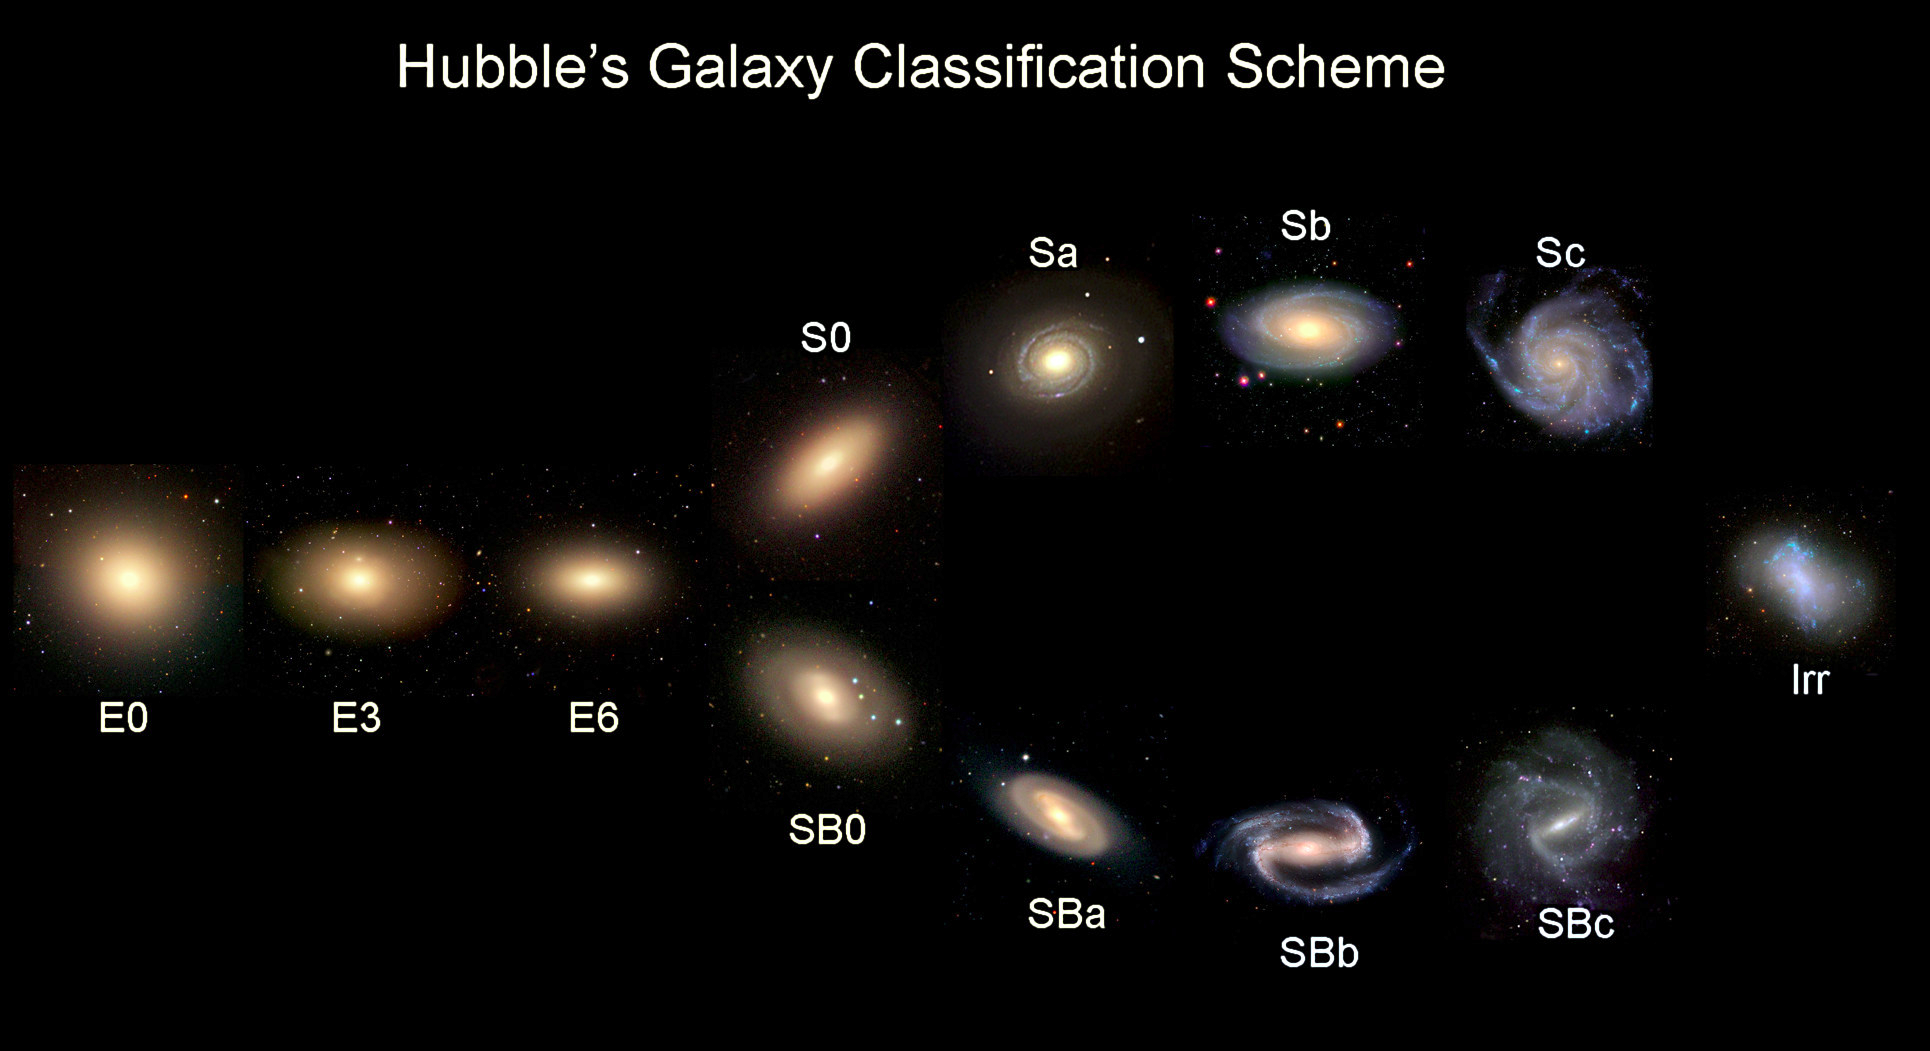
\includegraphics[width=\linewidth,trim={0 20mm 10mm 65mm},clip]{figures/hubble_sequence.png}
  \fonte{European Southern Observatory (ESO). Disponível em: \url{https://supernova.eso.org/exhibition/images/1015_fork-1920/}}
\end{figure}

% A importância da classificação morfológica na astronomia reside na sua capacidade de revelar padrões fundamentais sobre a evolução das galáxias e do universo como um todo. A morfologia galáctica não apenas reflete o estado atual de uma galáxia, mas também oferece pistas sobre sua história dinâmica, como colisões passadas, interações com outras galáxias e a presença de matéria escura. Por meio da classificação morfológica, os astrônomos podem investigar como as diferentes populações de galáxias variam ao longo do tempo cósmico, relacionando suas características estruturais com fatores como a densidade do ambiente e a quantidade de gás disponível para a formação estelar. Assim, a classificação morfológica se consolida como um método essencial para compreender a formação e evolução das galáxias, contribuindo para um entendimento mais profundo sobre a estrutura e a dinâmica do universo.








\section{Representação Morfológica por Ontologia}
\label{sec:ontologia}

\lipsum[1-2]









\section{Métodos de Classificação Morfológica}
\label{sec:classificao}

\lipsum[1]




\subsection{Anotação Manual por Especialistas}
\label{sec:classificacao-manual}

\lipsum[1-2]

No entanto, embora preciso, este método é ineficiente por conta da disparidade entre a capacidade de classificações manuais feitas por especialistas e a quantidade de objetos no Universo.




\subsection{Ciência Cidadã}
\label{sec:classificacao-cs}
Um método de classificação mais eficiente é a utilização da ciência cidadã, que é um campo interdisciplinar emergente que envolve a participação ativa do público geral em tarefas de pesquisas científicas com finalidade de produzir novos conhecimentos para a ciência e para a sociedade \cite{scs-1}, especialmente na coleta, categorização, transcrição e análise de dados científicos \cite{silvertown2009,bonney2014}. Este modelo de pesquisa tem ganhado relevância em diversos campos da ciência, principalmente devido ao aumento do acesso a tecnologias digitais e à internet, que facilitam a comunicação e a organização entre cidadãos e cientistas \cite{scs-4}.
%No decorrer dessa seção, será feito um breve levantamento do uso da ciência cidadã em diferentes áreas do conhecimento (Seção \ref{sec:cs-areas}), bem como na astronomia (Seção \ref{sec:cs-astro}), e uma perspectiva sobre a qualidade dos dados gerados (Seção \ref{sec:cs-data-quality}).

O GalaxyZoo\footnote{\url{https://galaxyzoo.org}} \cite{gz} é um projeto de ciência cidadã lançado em 2007, cujo objetivo é classificar morfologicamente galáxias utilizando imagens obtidas por grandes levantamentos astronômicos, como o Sloan Digital Sky Survey (SDSS). Os participantes, voluntários de diferentes formações e níveis de conhecimento científico, analisam imagens de galáxias e fornecem informações sobre suas características, como forma espiral, elíptica ou irregular, e a presença de estruturas específicas, como barras centrais. Essa colaboração massiva permitiu a classificação de milhões de galáxias em um curto período, superando em eficiência o que seria possível com equipes científicas tradicionais.

O impacto científico do GalaxyZoo é expressivo. Além de fornecer uma base de dados robusta e de alta qualidade para a pesquisa astronômica, o projeto gerou avanços no entendimento da formação e evolução de galáxias, incluindo a relação entre morfologia e ambiente. Os resultados têm sido utilizados para treinar modelos de aprendizado de máquina, permitindo a automação de tarefas de classificação em levantamentos futuros. O sucesso do GalaxyZoo também inspirou o desenvolvimento de outras plataformas de ciência cidadã, consolidando seu papel como ferramenta metodológica na pesquisa científica.

Para os voluntários, o GalaxyZoo oferece uma oportunidade de engajamento direto com a ciência, promovendo aprendizado e um senso de contribuição para descobertas científicas relevantes. Muitos participantes relatam um aumento na compreensão de conceitos astronômicos e motivação para explorar outras áreas da ciência. Além disso, a plataforma fomenta uma comunidade global de entusiastas que colaboram ativamente, monstando como iniciativas bem estruturadas podem democratizar o acesso e a participação no progresso científico.




\subsection{Métodos Computacionais}
\label{sec:classificacao-comp}

Os métodos computacionais atuais se baseiam nos métodos anteriores (Seções \ref{sec:classificacao-manual} e \ref{sec:classificacao-cs}) para treinamento de modelos.

\lipsum[1-2]

Este será o método explorado por este trabalho.












\chaptersep
